% AAMAS 2013 Manuscript

% This file should be compiled with "aamas2013.cls" 
% ----------------------------------------------------------------------
% REMEMBER: After having produced the .bbl file,
% and prior to final submission, you *NEED* to 'insert'
% your .bbl file into your source .tex file so as to provide
% ONE 'self-contained' source file.
% ----------------------------------------------------------------------

%%%%%%%%%%%%%%%%%%%%%%%%%%%%%%%%%%%%%%%%%%%%%%%%%%%%%%%%%%%%%%%%%%%%%%%%%%%%%%
% STYLE NOTES
%
% TENSE AND VOICE
% * Actual experimental events
% 	We wrote descriptions of actual experimental events using past tense, in 
%	active voice, as the first person plural.
%
% * All other contexts
%	We write all other text using present tense, in active voices, as the
%	the first person plural.  
%
% CONVENTIONS
% flapping-wing, small-scale, lightweight, MAV
%
%%%%%%%%%%%%%%%%%%%%%%%%%%%%%%%%%%%%%%%%%%%%%%%%%%%%%%%%%%%%%%%%%%%%%%%%%%%%%%
% SETUP
\documentclass{aamas2013}

%----------------------------------------------------------------------------%
% PACKAGES
\usepackage{color}
\usepackage[pdftex]{hyperref}
\usepackage{amsmath}

\newlength\eqnindent
\newlength\eqncolwid
\newcommand\eqntext[2][0pt]{%
  \setlength\parindent{0pt}%
      \setlength\eqnindent{#1}\setlength\eqncolwid{\linewidth}%
  \setlength\eqncolwid{\dimexpr\linewidth-\eqnindent}%
  \hspace*{\eqnindent}\parbox{\eqncolwid}{#2}%
}

%----------------------------------------------------------------------------%
% METADATA
\def \papertitle{Cooperative Control for Narrow Passage Traversal with an 
Ornithopter Micro Air Vehicle and Lightweight Ground Station}
\def \paperkeywords{AAMAS proceedings, multiagent systems, cooperative control, 
particle filter, micro air vehicle, ground station, visual servoing, pose 
estimation, flapping wing, ornithopter, biomimetic}
\def \paperterms{Algorithms, Performance, Design, Experimentation}
\def \paperauthors{Ryan C. Julian, Cameron J. Rose, Humphrey Hu, and Ronald S. Fearing}

% Set title
\title{\papertitle}

% PDF bookmarks
\definecolor{linkCol}{gray}{0.25}
\hypersetup{
    pdftitle={\papertitle},
    pdfauthor={\paperauthors},
    pdfsubject={\paperterms},
    pdfkeywords={\paperkeywords},
    pdfpagemode=UseOutlines, bookmarksopen, bookmarksnumbered,
    colorlinks, linkcolor=linkCol, citecolor=linkCol, urlcolor=linkCol
}

%----------------------------------------------------------------------------%
% pdfLatex clean-up 
\pdfpagewidth=8.5truein
\pdfpageheight=11truein

\begin{document}

%%%%%%%%%%%%%%%%%%%%%%%%%%%%%%%%%%%%%%%%%%%%%%%%%%%%%%%%%%%%%%%%%%%%%%%%%%%%%%
% AUTHORS

%% Paper number instead of authors
%\numberofauthors{1}
%\alignauthor Paper  580

\numberofauthors{4}
\author{
\alignauthor Ryan C. Julian\\
       \affaddr{Department of EECS}\\
       \affaddr{Univ. of California, Berkeley}\\
       \affaddr{Berkeley, CA 94720}\\
       \email{ryanjulian@berkeley.edu}
\alignauthor Cameron J. Rose\\
       \affaddr{Department of EECS}\\
       \affaddr{Univ. of California, Berkeley}\\
       \affaddr{Berkeley, CA 94720}\\
       \email{c\_rose@eecs.berkeley.edu}
\alignauthor Humphrey Hu\\
       \affaddr{Robotics Institute}\\
       \affaddr{Carnegie Mellon University}\\
       \affaddr{Pittsburgh, PA 15213}\\
       \email{humhu@cmu.edu}
\and
\alignauthor Ronald S. Fearing\\
       \affaddr{Department of EECS}\\
       \affaddr{Univ. of California, Berkeley}\\
       \affaddr{Berkeley, CA 94720}\\
       \email{ronf@eecs.berkeley.edu}
}

%%%%%%%%%%%%%%%%%%%%%%%%%%%%%%%%%%%%%%%%%%%%%%%%%%%%%%%%%%%%%%%%%%%%%%%%%%%%%%
% TITLE
\maketitle

%%%%%%%%%%%%%%%%%%%%%%%%%%%%%%%%%%%%%%%%%%%%%%%%%%%%%%%%%%%%%%%%%%%%%%%%%%%%%%
% ABSTRACT
\begin{abstract}
The power, size, and weight constraints of micro air vehicles (MAVs) limit 
their on-board sensing and computational resources. Ground vehicles have 
less mobility than MAVs, but relaxed size constraints and typically more 
computing power, creating opportunities for cooperation. In this work, we 
demonstrate cooperative target-seeking between a 13 gram ornithopter MAV 
and a lightweight ground station using computer vision.

We also introduce a new ornithopter MAV, the 13 gram H$^2$Bird. It 
features clap and fling wings, improves upon a previous design by 
utilizing a carbon fiber airframe, tail rotor, and elevator, and carries a 
payload of 2.8 grams. We augment the ornithopter's built-in 
gyroscope-based control with a ground station, which has power and weight 
requirements appropriate for deployment on 30 gram a ground vehicle. The ground 
station provides heading estimates to the ornithoper by running a 
real-time motion tracking algorithm on a live video stream. This allows 
the ornithopter to reliably negotiate flight through narrow openings.

We demonstrate the performance of the location estimation and navigation 
algorithms. We model the backwards-reachable region for successfully 
navigating through narrow openings. Finally, we verify this model through 
with collected in experiments with narrow passage traversal.
\end{abstract}
%%%%%%%%%%%%%%%%%%%%%%%%%%%%%%%%%%%%%%%%%%%%%%%%%%%%%%%%%%%%%%%%%%%%%%%%%%%%%%
% ACM METADATA

% Note that the category section should be completed after reference to 
% the ACM Computing Classification Scheme available at
% http://www.acm.org/about/class/1998/.
% A category including the fourth, optional field follows...
%\category{D.2.8}{Software Engineering}{Metrics}[complexity measures, 
% performance measures]
\category{I.2.9}{Robotics}{Autonomous Vehicles}
\category{I.2.9}{Robotics}{Distributed Artificial Intelligence}[Multiagent Systems]
\category{I.2.9}{Robotics}{Vision and Scene Understanding}[Motion]

% General terms should be selected from the following 16 terms: 
% Algorithms, Management, Measurement, Documentation, Performance, 
% Design, Economics, Reliability, Experimentation, Security, 
% Human Factors, Standardization, Languages, Theory, Legal Aspects, 
% Verification.
\terms{\paperterms}

% Keywords are your own choice of terms you would like the paper to be indexed 
% by.
\keywords{\paperkeywords}

%%%%%%%%%%%%%%%%%%%%%%%%%%%%%%%%%%%%%%%%%%%%%%%%%%%%%%%%%%%%%%%%%%%%%%%%%%%%%%
\section{Introduction}
%TODO ryan
\begin{figure}[!tb]
\centering
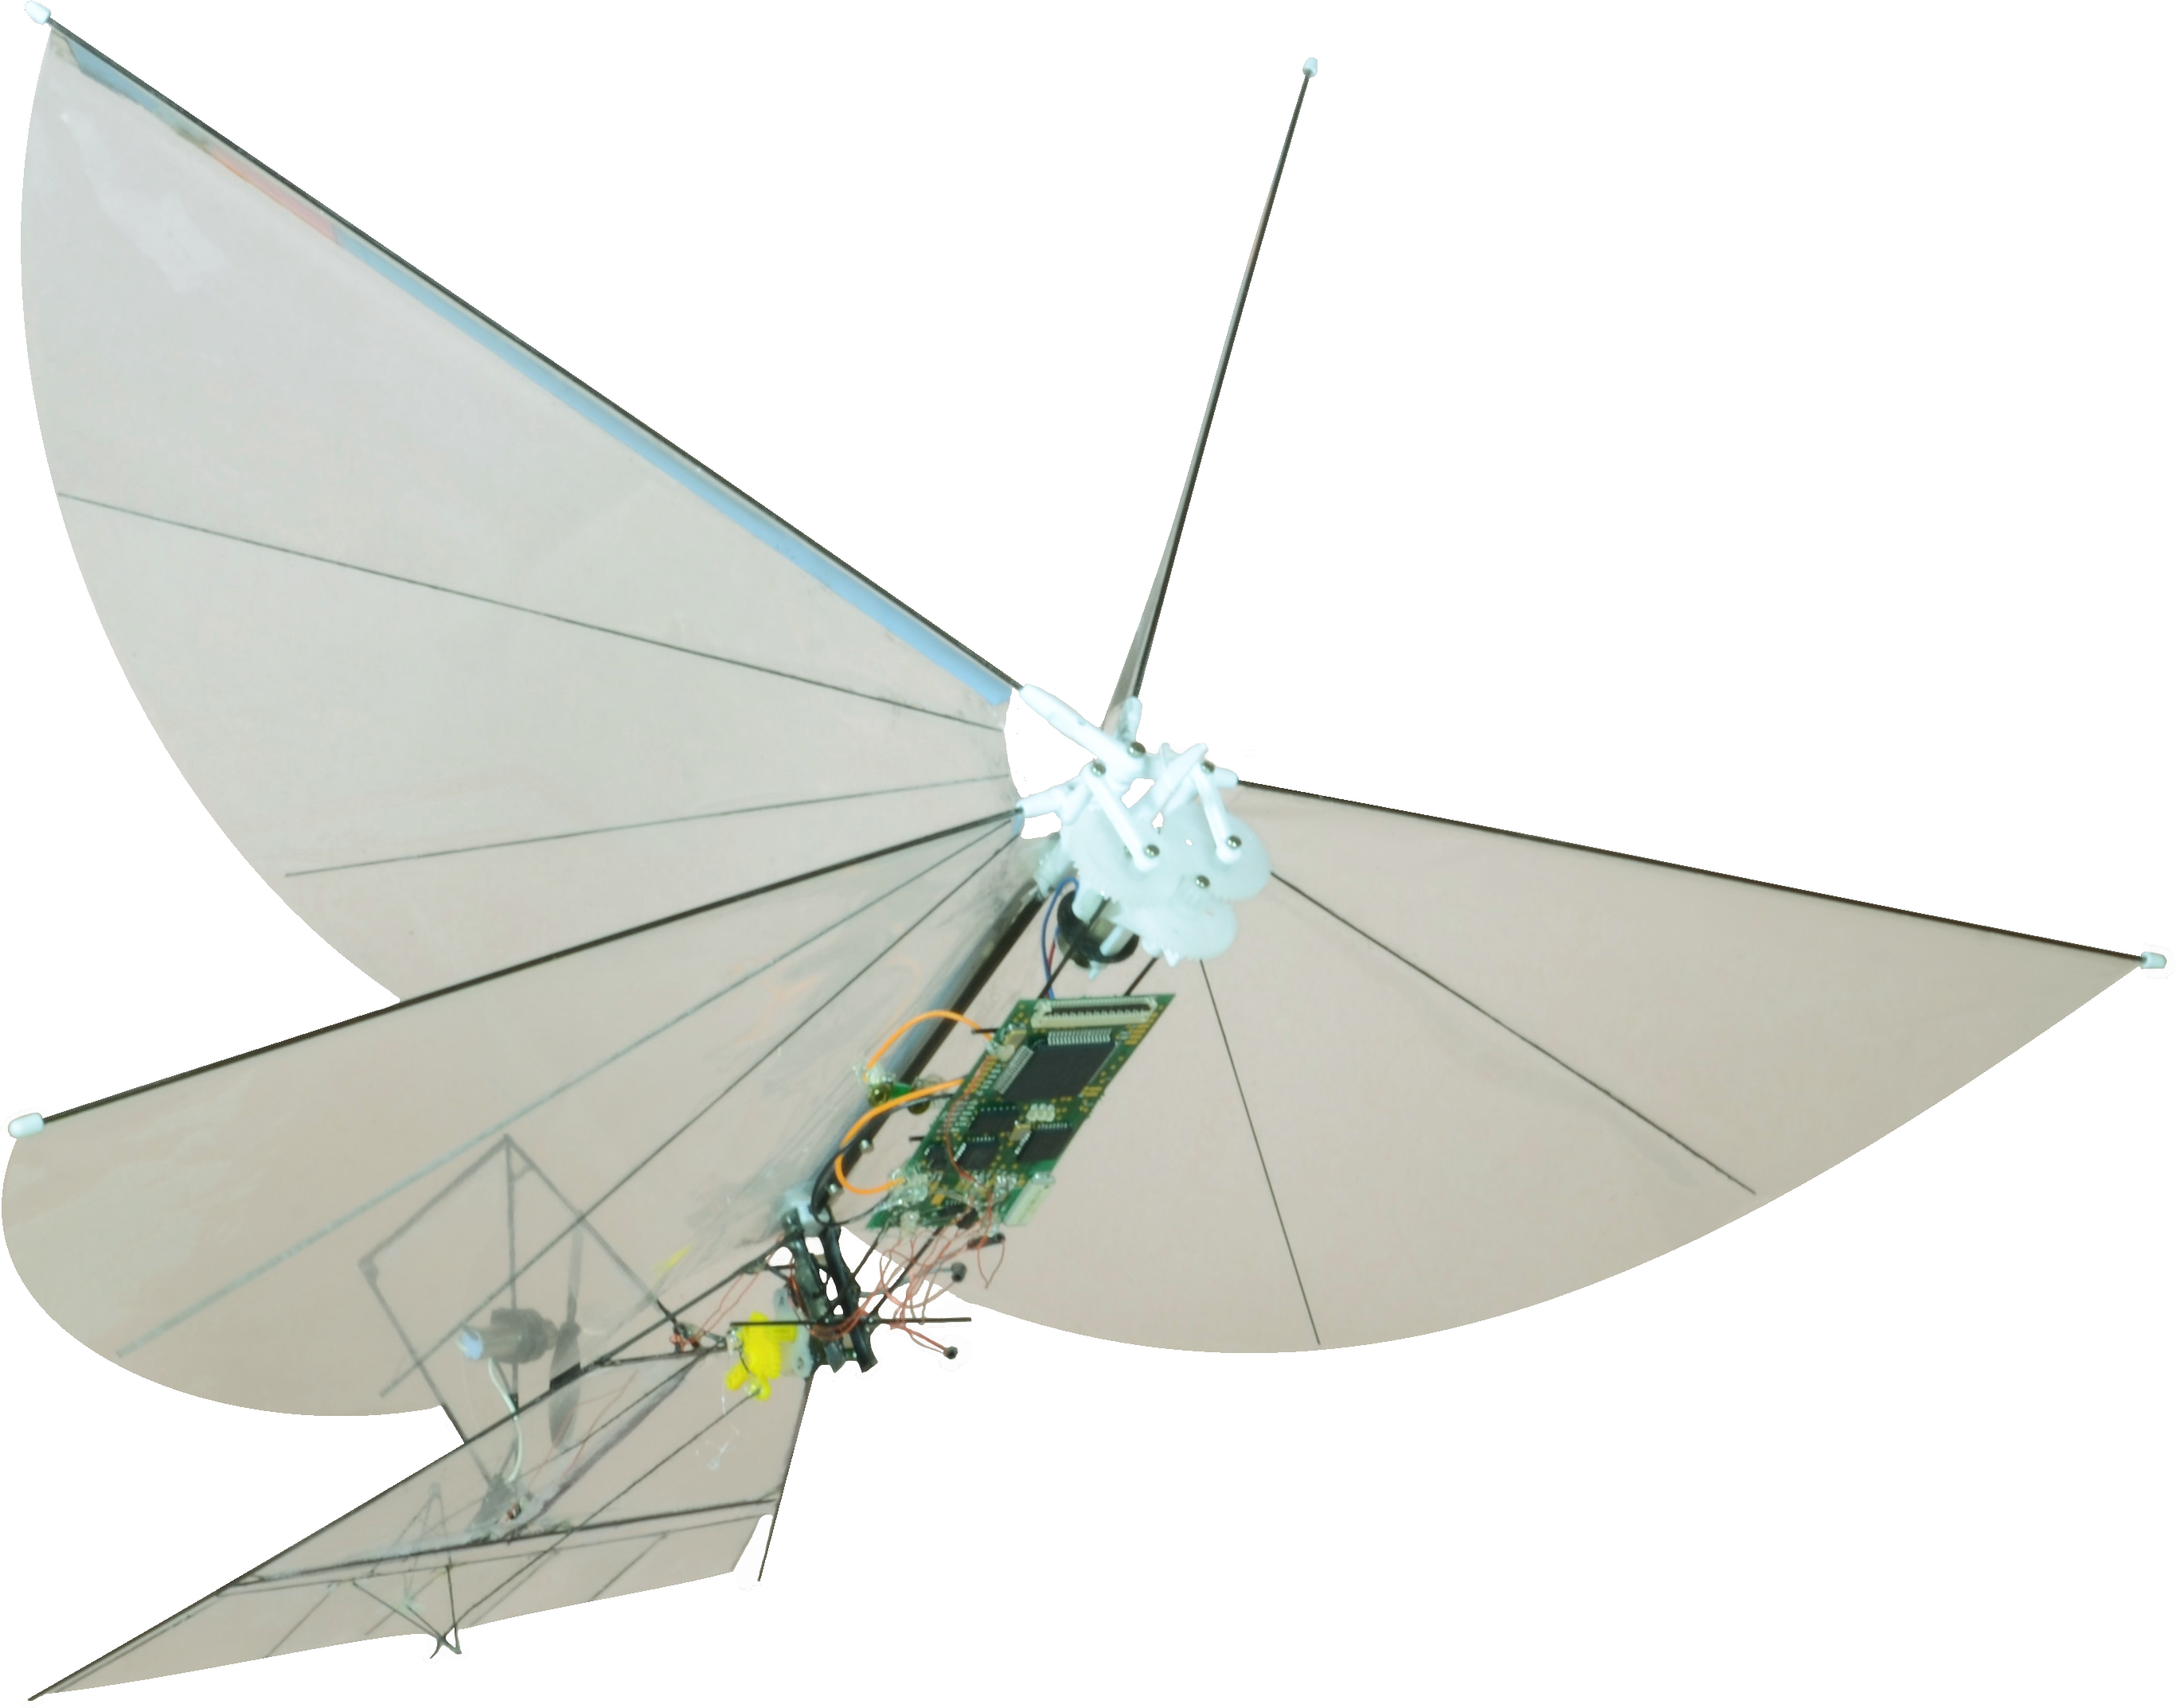
\includegraphics[width=\linewidth]{figures/h2bird.png}
\caption{H$^2$Bird ornithopter MAV}
\label{fig:h2bird}
\end{figure}
The power, size, and weight constraints of micro air vehicle (MAV) 
platforms significantly limit on-board sensing and computational 
resources, and thus the complexity of the control and state estimation 
algorithms which can be executed on-board. These constraints are 
particularly severe for flapping wing MAVs, a class of MAVs that have inherently superior 
safety, efficiency, and noise profile to rotor craft MAVs, but at the 
expense of payload weight.
%Intro portion about previous works in ornithopter coorperative control/
%modeling ( won't necessarily stay in this spot)
Modeling and control of flapping wing MAVs is a well studied subject. 
Shigeoka discusses velocity and altitude control in
~\cite{Shigeoka:ornithopter}. In~\cite{delfly:design} deCroon et al. %TODO sentence fragment
In contrast, there is little previous work on guidance of flapping wing 
MAVs. Baek demonstrated altitude control with an external 
camera~\cite{baek:altitude}. de Croon et al. demonstrated obstacle avoidance 
with an onboard camera and offboard processing~\cite{delfly:avoid}. 
%[However, these papers do not study the system blah blah blah.]

Autonomous control of flapping winged MAVs is a complex undertaking because of
the non-linear flight dynamics as presented
in~\cite{humbert:dipteran2}\cite{cheng:tandrdamping}. Although the dynamics of
flapping-winged flight can be averaged with respect to the wingbeat period as
presented in~\cite{Schenato:flightcontrol}\cite{cheng:tandrdamping}, we develop a
linear, one-dimensional model to predict the behavior of the system, similar
to~\cite{Shigeoka:ornithopter}. In addition to the nonlinearities, the system
is underactuated due to size constraints. Many of the methods for controlling
these platforms make extensive use of GPS in outdoor
environments~\cite{kingston:timeattitude, kanade:3dvision} and expansive
motion capture systems in indoor environments. While operating indoors, using
GPS to estimate the pose of the MAV is not possible, and motion capture
requires expensive and stationary modification of the environment. The power
and payload limits on MAVs make on-board sensing difficult, so multi-agent
cooperative control schemes are apt solutions.

Many of the control laws that previous researches have developed from the
dynamic models of flapping-winged flight, such as periodic forcing and other
control methods as described %TODO you need to use real names, it's not kosher to refer to citation numbers directly
in~\cite{doman:dynamics}\cite{khan:longitudinal_control}\cite{leonard:averaging}, are computationally complex and
require powerful on-board computing. In our work, we develop a simpler, less
computationally intensive method of control for negotiating narrow passages.

%%%%%%%%%%%%%%%%%%%%%%%%%%%%%%%%%%%%%%%%%%%%%%%%%%%%%%%%%%%%%%%%%%%%%%%%%%%%%%
\section{Robotic and Vision Platforms}
%TODO ryan

%----------------------------------------------------------------------------%
\subsection{H$^2$Bird Ornithoper}
% humphrey
In order to conduct these experiments on cooperation, we designed a new
flapping-wing MAV, known as the H$^2$Bird. Built around the Silverlit I-Bird 
RC flyer power train and clap-fling 
wings\footnote{\url{http://www.silverlit-flyingclub.com/wingsmaster/}}, 
the H$^2$Bird's wingspan is 26.5 cm and it has a flight weight of 13 grams. A 
tail propeller and servo-controlled tail elevator provide control in the yaw 
and pitch axes. The on-board ImageProc 2.4\footnote{Expand! Accredit it to Stan Baek!} 
electronics package consists of a 40 MIPS microprocessor, 6 DOF IMU, 
IEEE 802.15.4 radio, VGA camera, and motor drivers, all powered by a 90 mAh 
lithium polymer battery. In routine flight, the H$^2$Bird averages 1.2 m/s 
ground speed, and can operate for approximately 10 minutes.
%TODO footnote for ImageProc

%----------------------------------------------------------------------------%
\subsection{Ground Station Computer Vision Platform}
% ryan
Cooperative behavior is a promising strategy for autonomous navigation of 
unexplored and unstructured environments. We intend that this system will be 
fully mobile in these environments, not tied to a static ground station or 
motion capture laboratory. To demonstrate the feasibility of this approach, 
we designed our ground station to conform to the power and weight 
constraints of highly mobile millirobotic ground vehicles, such as 
OctoRoACH, which can traverse rough terrains with speed and agility [CITATION]. 
%TODO OctoRoACH citation

Rather than power-intensive PC processors, we used the ARM-based 
BeagleBoard single-board computer as reference computation platform. The
BeagleBoard consumes approximately 1 watt while running our computer vision 
and control algorithms. It uses the same processor as popular sub-10 gram 
processor modules--such as the Gumstix Overo and LogicPD Torpedo--which are 
light enough for deployment on millirobotic ground vehicles. We pair the 
BeagleBoard with an off-the-shelf consumer USB web camera, for similar image 
quality and resolution to the miniature camera modules available at 
millirobot scale. The BeagleBoard communicates with the H$^2$Bird using a 
USB radio module which implements the IEEE 802.15.4 wireless standard.
%TODO footnotes: Gumstix, LogidPD

Our ground station software is based on the Ubuntu Linux distribution, 
modified with a custom version of the Linux kernel. We use the Python 
programming language for control, robot communication, and telemetry, and 
the OpenCV computer vision libraries for image capture and processing.
%TODO footnotes: Ubuntu, Linux, Python, OpenCV
%%%%%%%%%%%%%%%%%%%%%%%%%%%%%%%%%%%%%%%%%%%%%%%%%%%%%%%%%%%%%%%%%%%%%%%%%%%%%%
\section{System Concept and Algorithms}
%TODO ryan

\begin{figure}[tb]
\centering
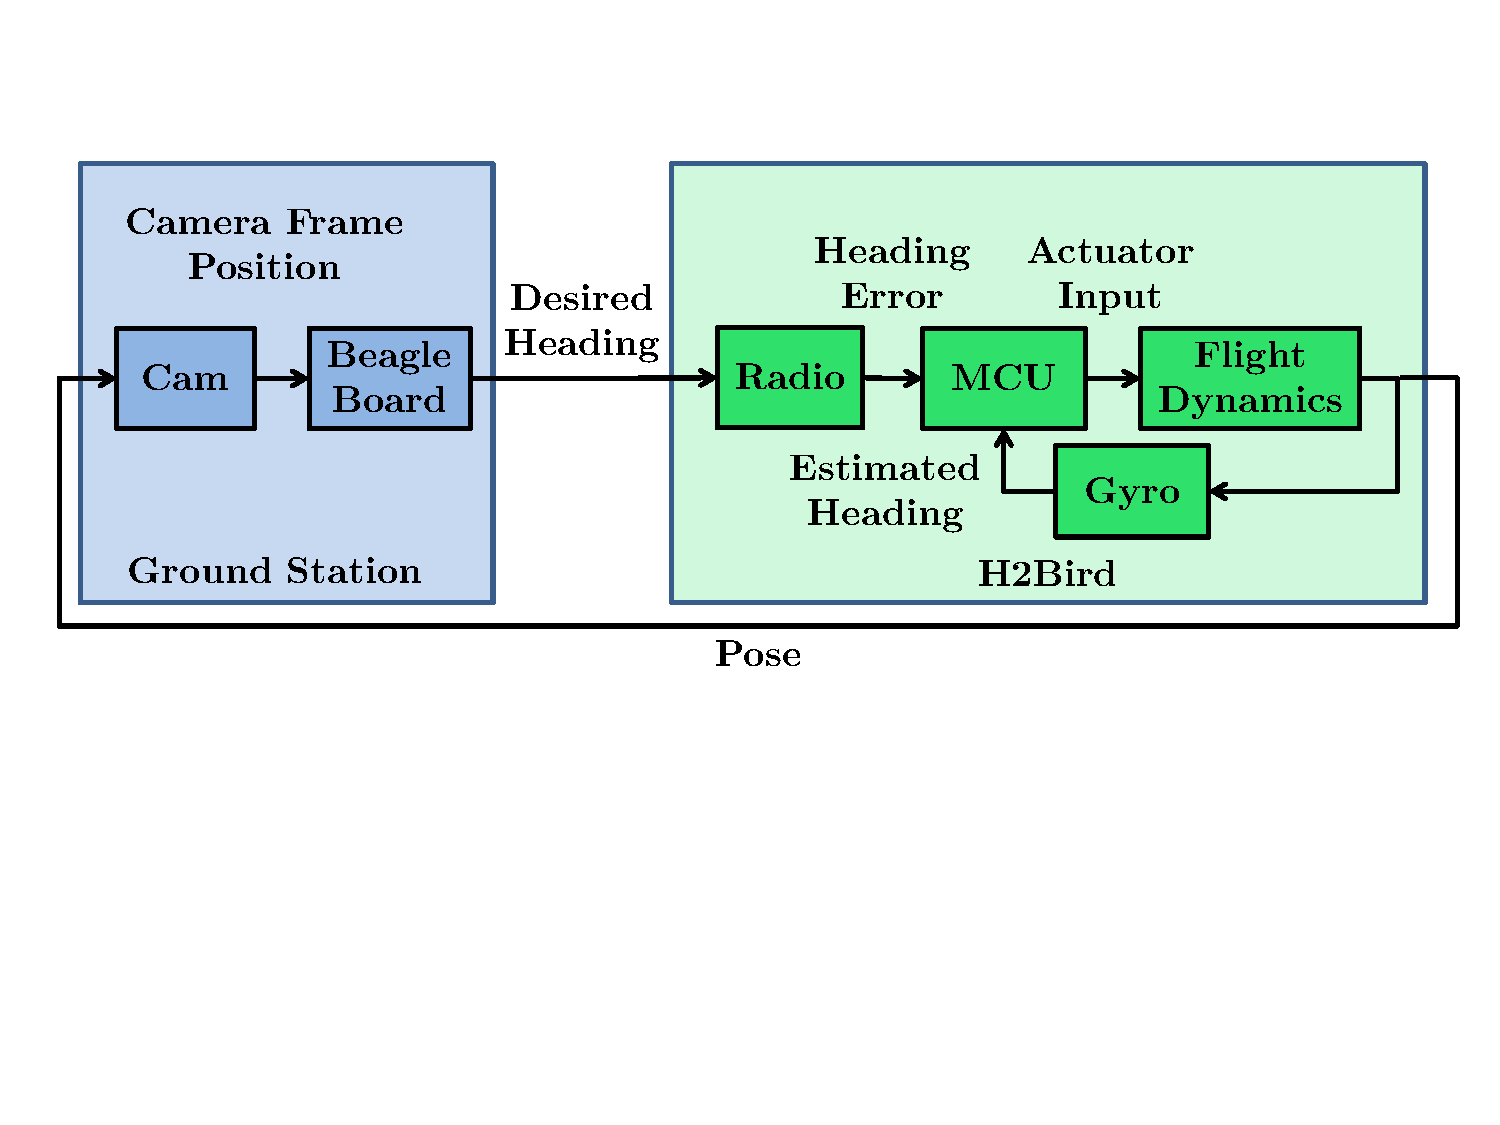
\includegraphics[width=\linewidth]{figures/process_flow.pdf}
\caption{Overview of the cooperative control system.}
\label{fig:process_flow}
\end{figure}
%TODO h2bird label in diagram should have superscript

%----------------------------------------------------------------------------%
\subsection{Ornithoper Attitude Control}

\begin{figure}[!tb]
\centering
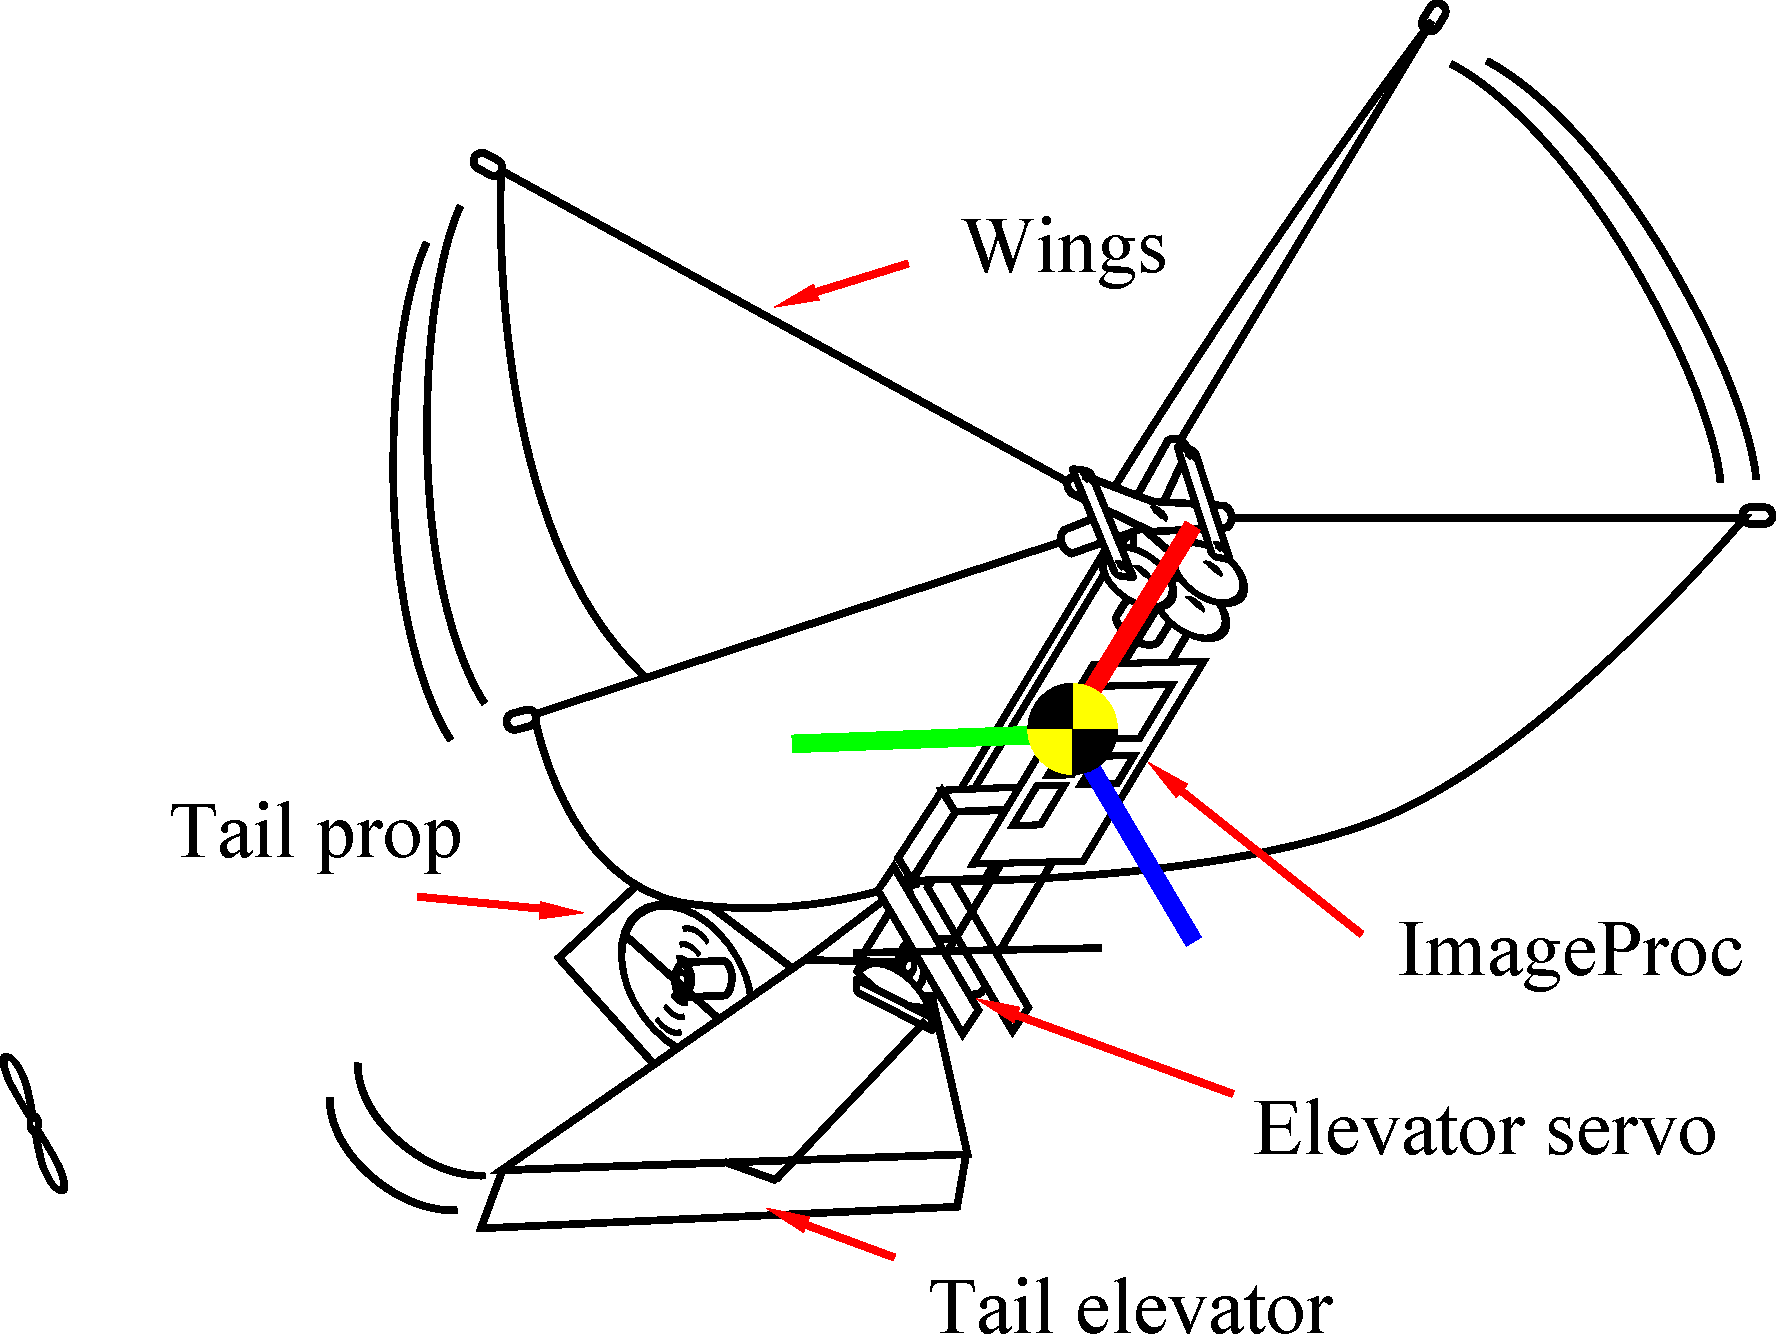
\includegraphics[height=150pt]{figures/h2bird_axes.pdf}
\caption{H$^2$Bird ornithopter with attitude control axes and labeled control surfaces.}
\label{fig:h2Bird_axes}
\end{figure}
%TODO label h2bird drawing

Attitude estimation and control for the H$^2$Bird runs on-board to achieve 
maintain high-rate attitude control. We estimate the vehicle pose by naively
integrating the IMU, and use PID for controlling the vehicle.

The high pitch angles H$^2$Bird achieves in routine flight distinguishes it 
from other MAVs. Baek 
demonstrated control on a similar vehicle using PID and an Euler angle
parameterization of orientation~\cite{baek:tracking}. However, Euler angle parameterizations of the vehicle orientation 
suffer from singularities around these high pitch angles, so we instead 
represent the vehicle orientation with quaternions. An additional benefit of 
the quaternion representation its ability to represent relative body and 
world coordinate angular displacements compactly with quaternion 
multiplication.

Our implementation of quaternion-based control is similar to Knoebe's~\cite{knoebe:quatcontrol}:
Given a reference quaternion $q$, we define the error $q_e$ as the rotation 
required to reach the reference pose from the measured pose (Eq.~\ref{eq:quat_error}). 
\begin{equation}
\label{eq:quat_error}
q_e = q'\otimes q_r
\end{equation}
We then convert this error quaternion to an angle axis, and use this 
representation as input to the PID controller 
(Eqs.~\ref{eq:quat_angle} and~\ref{eq:quat_linearize}). 
\begin{equation}
\label{eq:quat_angle}
\alpha = 2\arccos(q_{e,w})
\end{equation}
\begin{equation}
\label{eq:quat_linearize}
Q_e = \alpha*q_e/\sin(\alpha /2)
\end{equation}

%----------------------------------------------------------------------------%
\subsection{Ground Station Pose Estimation}
%TODO ryan
The ground station performs simple two-dimensional pose estimation on 
H$^2$Bird using a particle filter-based motion tracking algorithm. This pose 
estimate is the feedback input to the cooperative visual servoing feedback 
loop (Sec. \ref{sec:visual_servoing_concept}). We limit our pose estimation 
approach to monocular two-dimensional object tracking in pixel space. This 
allows us to perform real-time video tracking using the modest computational 
resources available on the ground station, and similarly millirobotic ground 
vehicles.

Our pose estimation algorithm tracks H$^2$Bird motion in the frame using a 
particle filter~\cite[96-114]{thrun2005probabilistic}. We initialze particles 
uniformly across the frame. To improve numerical stability, we  normalize the 
weights of all particles on each iteration, and only resample the particle 
population when the mean particle weight falls below a pre-determined 
threshold.

%............................................................................%
\subsubsection{Motion Model}
Our motion model (Eq.~\ref{eq:motion_model}) is a simple Gaussian transition 
centered around each particle's current position, augmented with an 
$\epsilon$-random uniform sampling strategy. In Eq.~\ref{eq:motion_model}, 
$x^{[i]}_t$ is the state of the $i^\text{th}$ particle at time $t$, $\Sigma$ 
is a chosen covariance matrix, and $b$ is vector of the height and width of 
the camera frame.
\begin{equation}
\label{eq:motion_model}
x^{[i]}_t \sim \begin{cases}
\mathcal{N}(x^{[i]}_{t-1}, \Sigma), &\text{with probability } 1-\epsilon \\
\mathcal{U}(0,b),& \text{with probability } \epsilon \\
\end{cases}\\
\end{equation}
The experiments presented in this paper used a diagonal covariance matrix 
with variance 256, and an $\epsilon$ of 0.3. We find that the Gaussian 
transition model is sufficient for tracking motion in which frame-to-frame 
position changes are relatively small. The $\epsilon$-random uniform 
transitions increase tracking robustness, by forcing the filter to always 
sample all of the pixel space. This prevents overconfidence and collapse, 
and decreases reacquisition delay. 

%............................................................................%
\subsubsection{Emission Model}

%----------------------------------------------------------------------------%
\subsection{Cooperative Visual Servoing}
\label{sec:visual_servoing_concept}

\begin{figure}[tb]
\centering
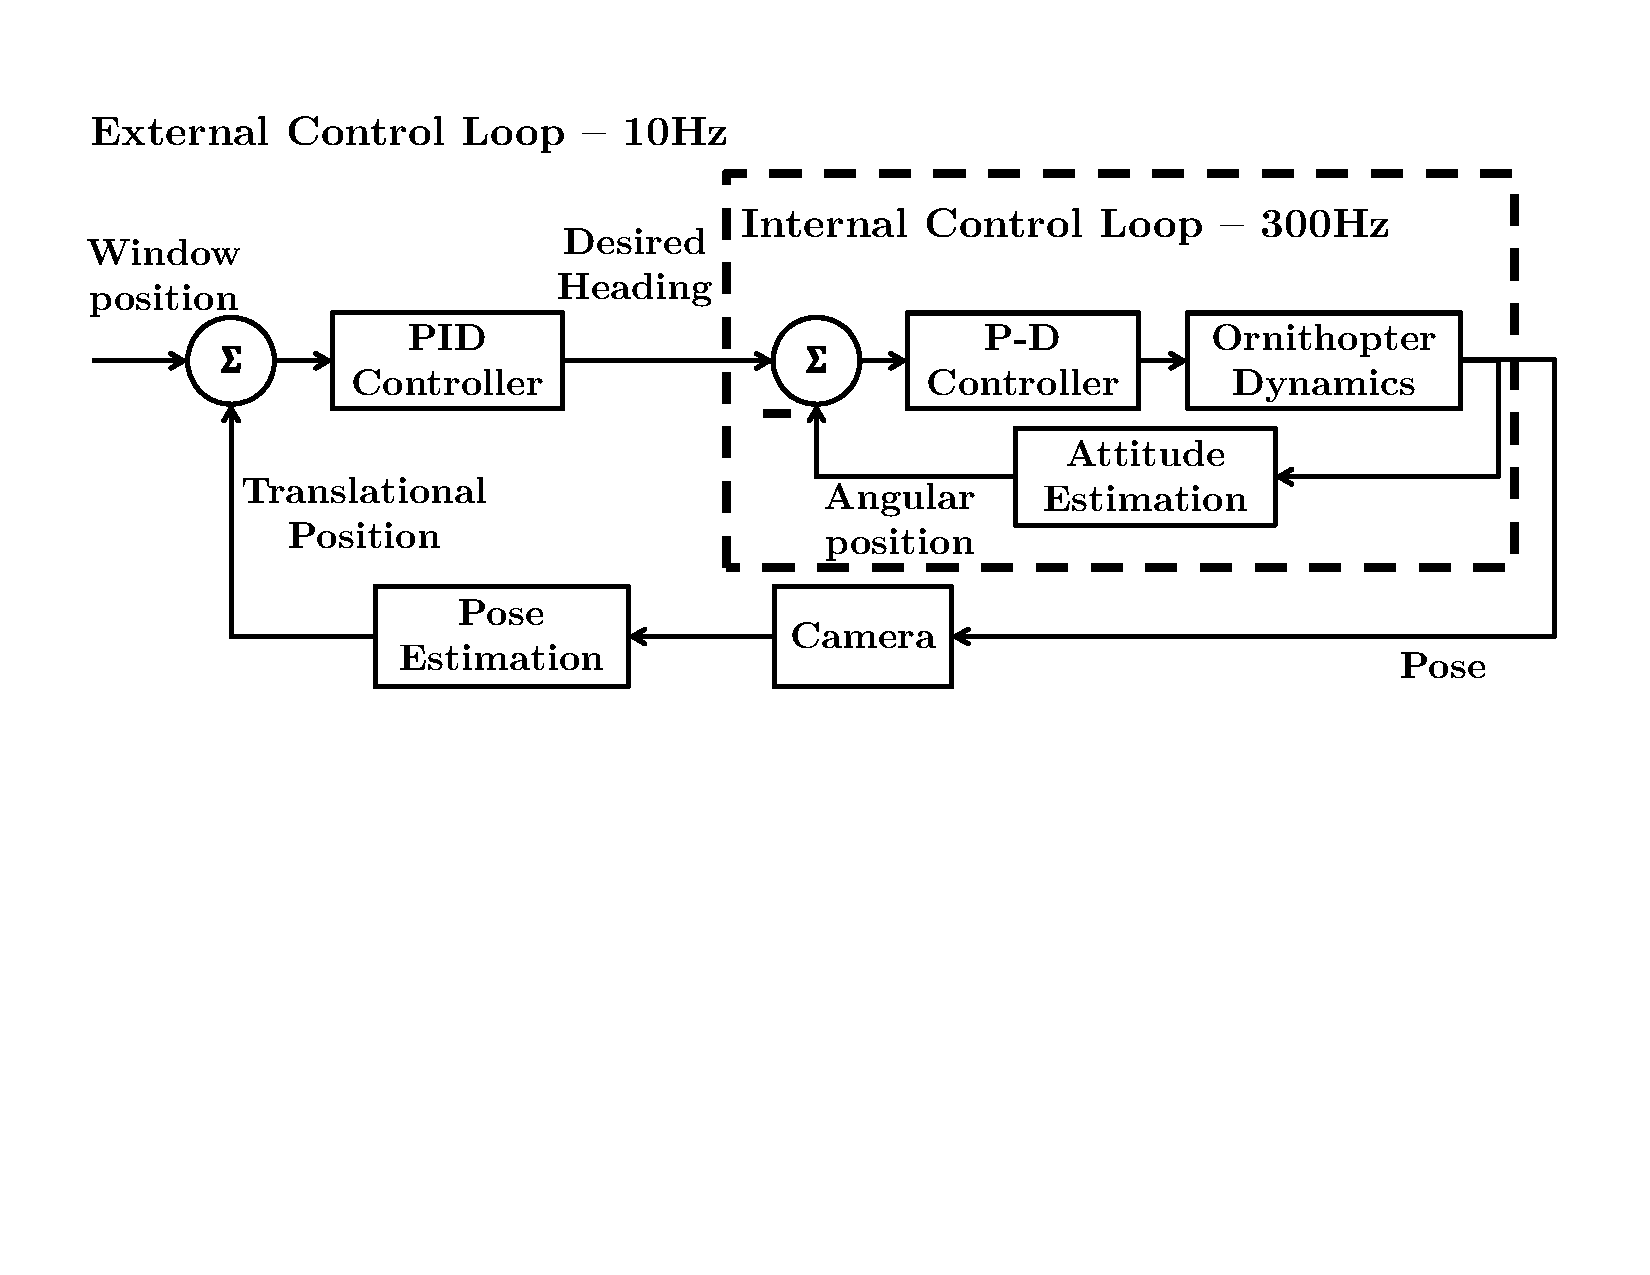
\includegraphics[width=\linewidth]{figures/block_diagrams.pdf}
\caption{Overall block diagram of the cooperative control system.}
\label{fig:block_diagram}
\end{figure}

\begin{figure}[tb]
\centering
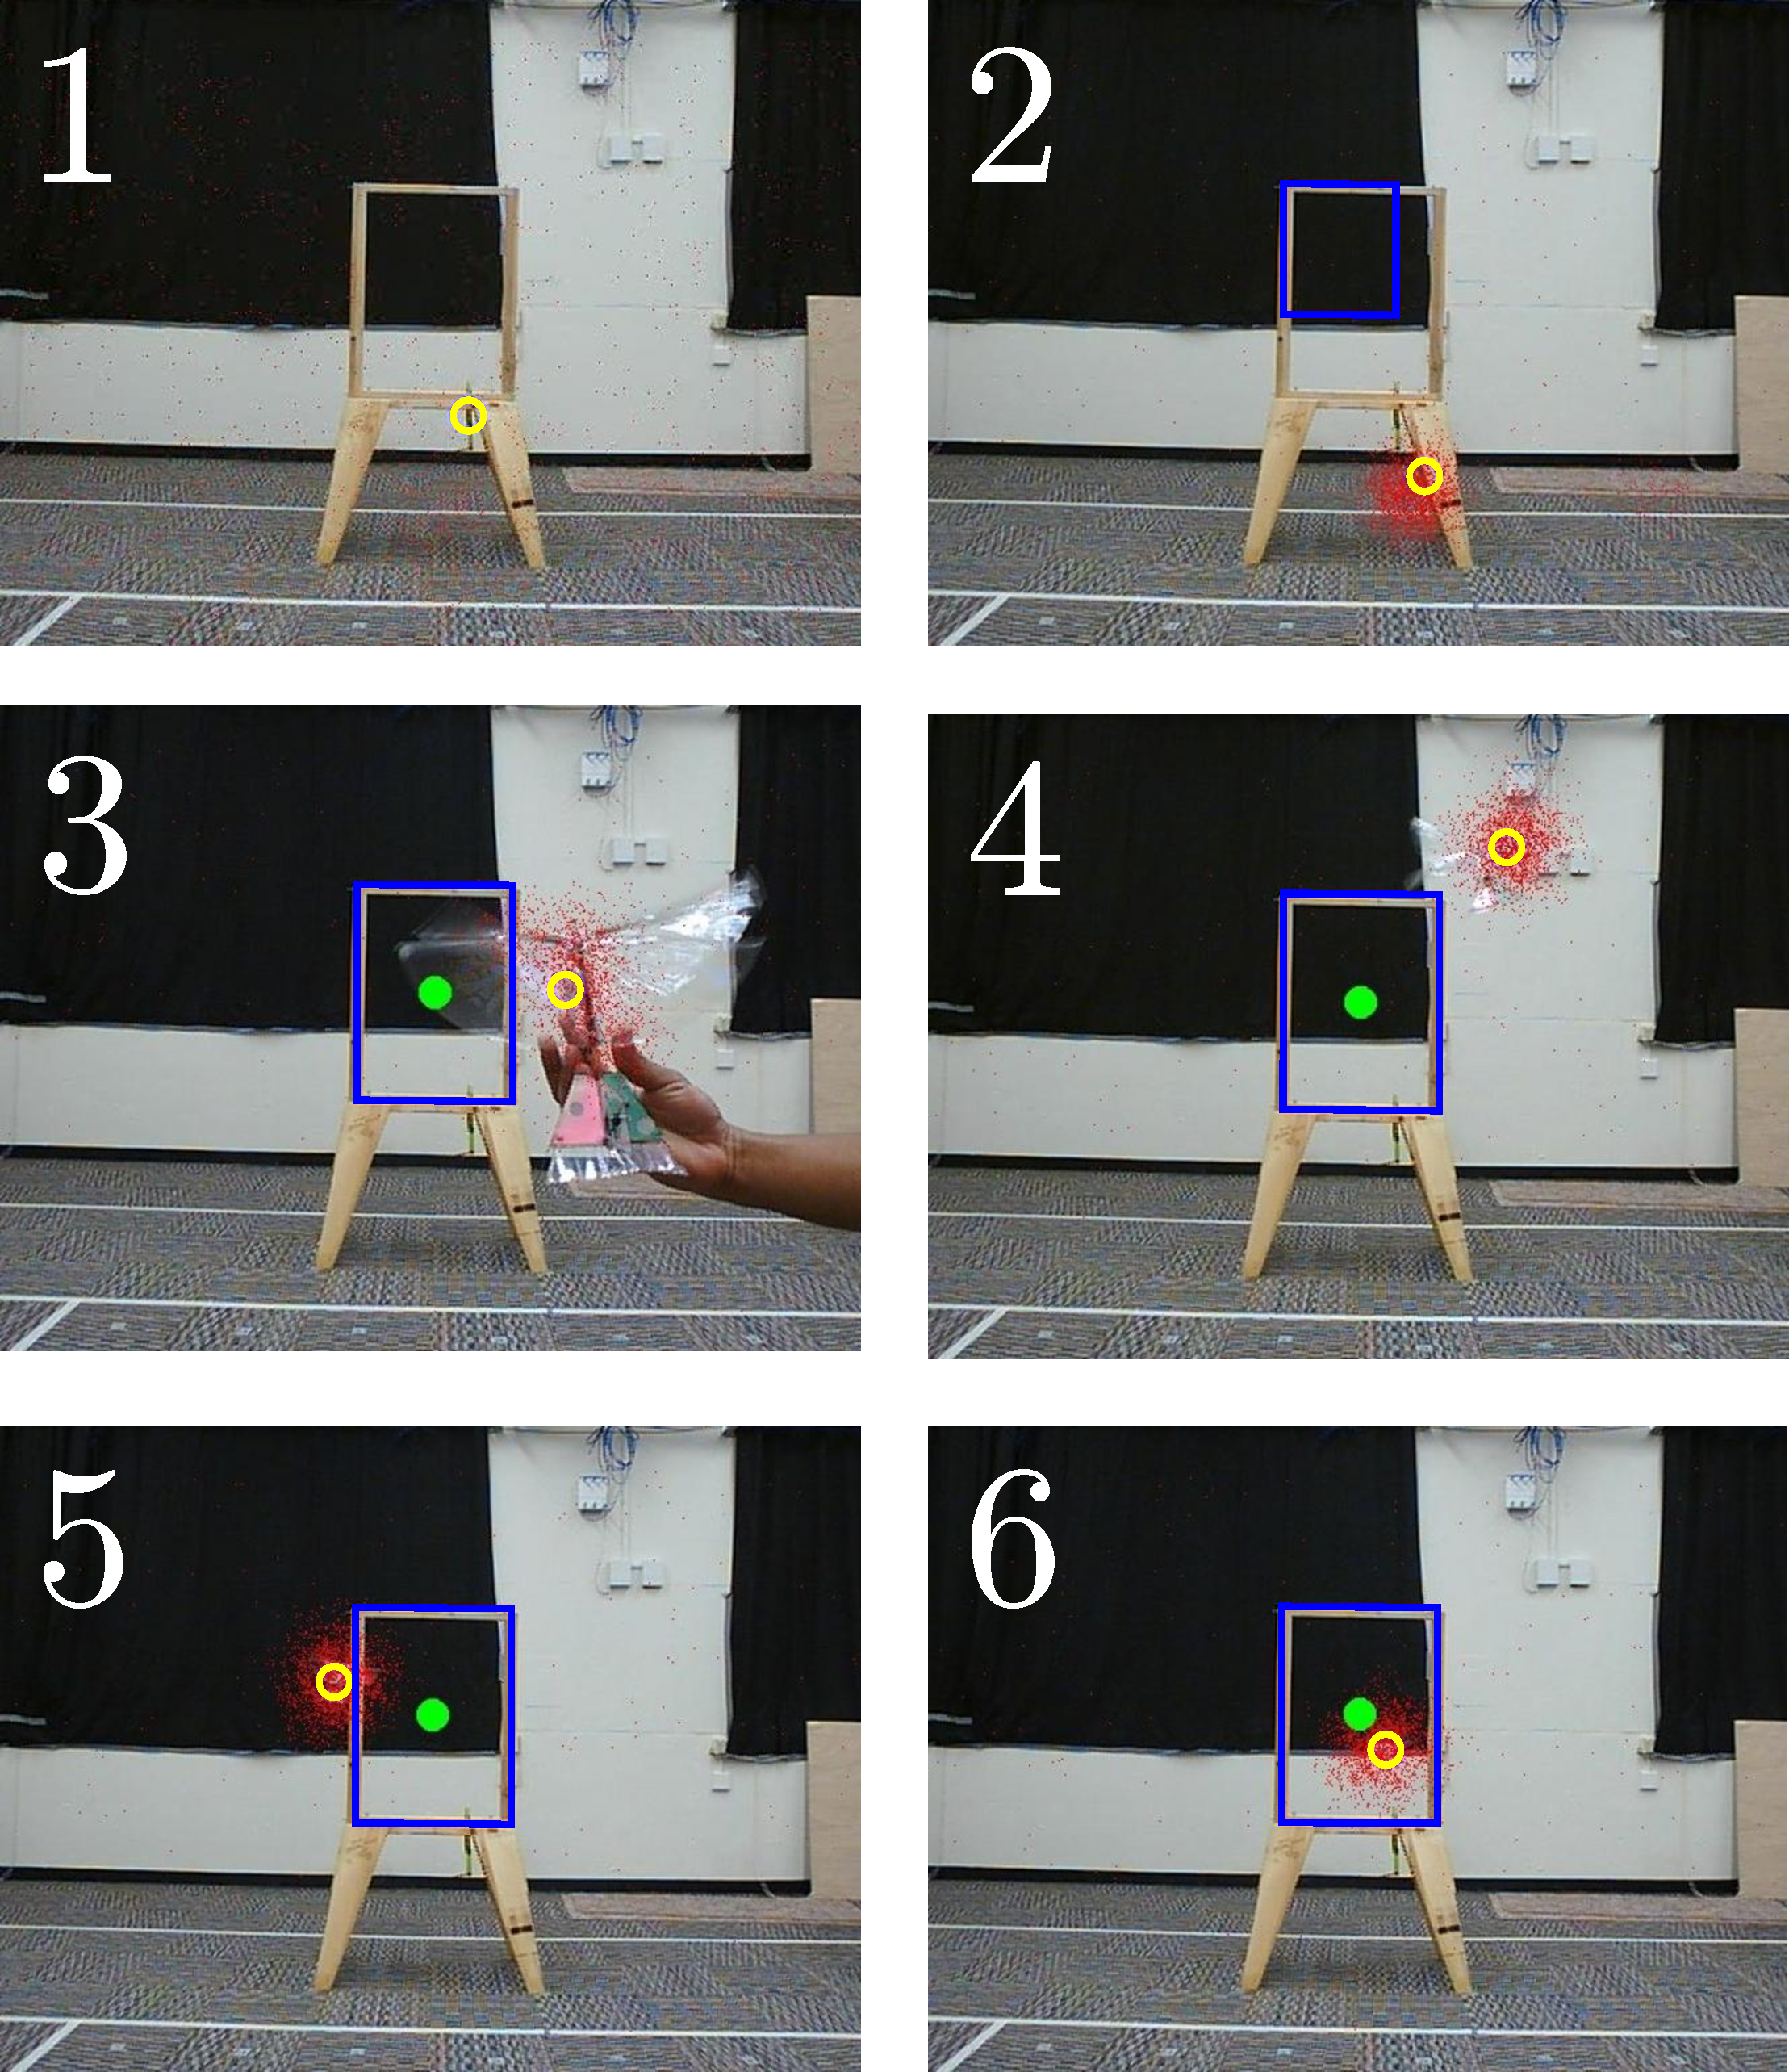
\includegraphics[width=\linewidth]{figures/pf_screencap.pdf}
\caption{Frame sequence from video feed used for tracking. Particles 
are shown in \textcolor{red}{red}, the current state estimate as a 
\textcolor{blue}{blue} circle, the window bounding box in
\textcolor{red}{red}, and the target location as a \textcolor{green}{green} 
circle. 1.~Particles initialized uniformly across the frame; 2.~Human operator 
dragging bounding box across the window; 3.~H$^2$Bird enters the frame. 
Particles converge on its location; 4.~Release H$^2$Bird, which 
begins cooperative autonomous flight toward the target; 5.~Visual servoing 
controller overshoots the window on the left, and commands a right-turn 
maneuver to recover; 6.~H$^2$Bird successfully navigates through the window.}
\label{fig:pf_screencap}
\end{figure}

%%%%%%%%%%%%%%%%%%%%%%%%%%%%%%%%%%%%%%%%%%%%%%%%%%%%%%%%%%%%%%%%%%%%%%%%%%%%%%
\section{System Model}
\label{sec:system_model}

%----------------------------------------------------------------------------%
\subsection{Ornithopter Attitude Control}

We gathered the data for the experiment by integrating the output of
H$^2$Bird's on-board gyroscope data. We then used
MATLAB\footnote{\url{http://www.mathworks.com/products/matlab/}} to fit a
simple low-order model (Eq.~\ref{eq:transfer_func}) of the turning
behavior to the step response with the physical heading as the state and the
heading set point as the input. This model serves as a simplification of both
the turning dynamics of the ornithopter and the on-board PID-based attitude
controller. We use this model in Section~\ref{sec:visual_servoing} to
determine the backwards reachable region for navigating through narrow
passages.

%----------------------------------------------------------------------------%
\subsection{Ground Station Pose Estimation}

%----------------------------------------------------------------------------%
\subsection{Cooperative Visual Servoing}

%%%%%%%%%%%%%%%%%%%%%%%%%%%%%%%%%%%%%%%%%%%%%%%%%%%%%%%%%%%%%%%%%%%%%%%%%%%%%%
\section{Experiments}

%----------------------------------------------------------------------------%
\subsection{System Identification}

%............................................................................%
\subsubsection{Ornithoper Attitude Control}

We determined the turning speed and turning radius of the H$^2$Bird
experimentally using the response of the system to the step input of a
clockwise 90 degree turn. To measure the response of the system, we recorded
the angular position data of the ornithopter calculated from the on-board
gyroscope data.

%............................................................................%
\subsubsection{Ground Station Pose Estimation}

%............................................................................%
\subsubsection{Cooperative Visual Servoing}

%----------------------------------------------------------------------------%
\subsection{Model Verification}

We tested our cooperative visual servoing system with a simple target seeking
experiment: the H$^2$Bird must fly through a specified obstacle, in this case,
a wooden frame meant to simulate a window. As the H$^2$Bird cannot detect the
target on its own,we used the ground station to provide remote headings for
navigation to the window. Ground truth data was collected via a motion capture
system in the test room. A sketch of the experimental setup is shown in
Fig.~\ref{fig:experiment_cartoon}.

% TODO clarify or roll into paragraph
Each trial included the following steps:
\begin{enumerate}
\item The window is identified by the user. 
\item The H$^2$Bird is released in view of the camera by hand at the desired starting grid point.
\item The H$^2$Bird attempts to fly to the window with remote guidance from
the base station.
\end{enumerate}

In total, 80 trials were run over a variety of starting positions. The goal of our experiments was to verify the model described in~\ref{sec:system_model}, so we conducted 60 of the 80 trials in a grid along the edges of the camera viewplane in 0.05 meter increments from the window to determine the success rate on the edges of the testing space. We conducted 20 additional trials directly in front of the camera to determine the success rate near the center of the testing space. The H$^2$Bird battery was changed approximately every 5 tests, adding more variation to the H$^2$Bird performance by affecting the motor power output.

% Don't think this goes here
Variations in the H$^2$Bird hand launch caused the system to respond 
differently for similar initial conditions. In addition, the H$^2$Bird 
battery was changed approximately every 5 tests, adding more variation to
the H$^2$Bird performance by affecting the motor power output. The effects of 
these noisy factors is considered in Section ~\ref{sec:performance}.
% Might move

\begin{figure}[tb]
\centering
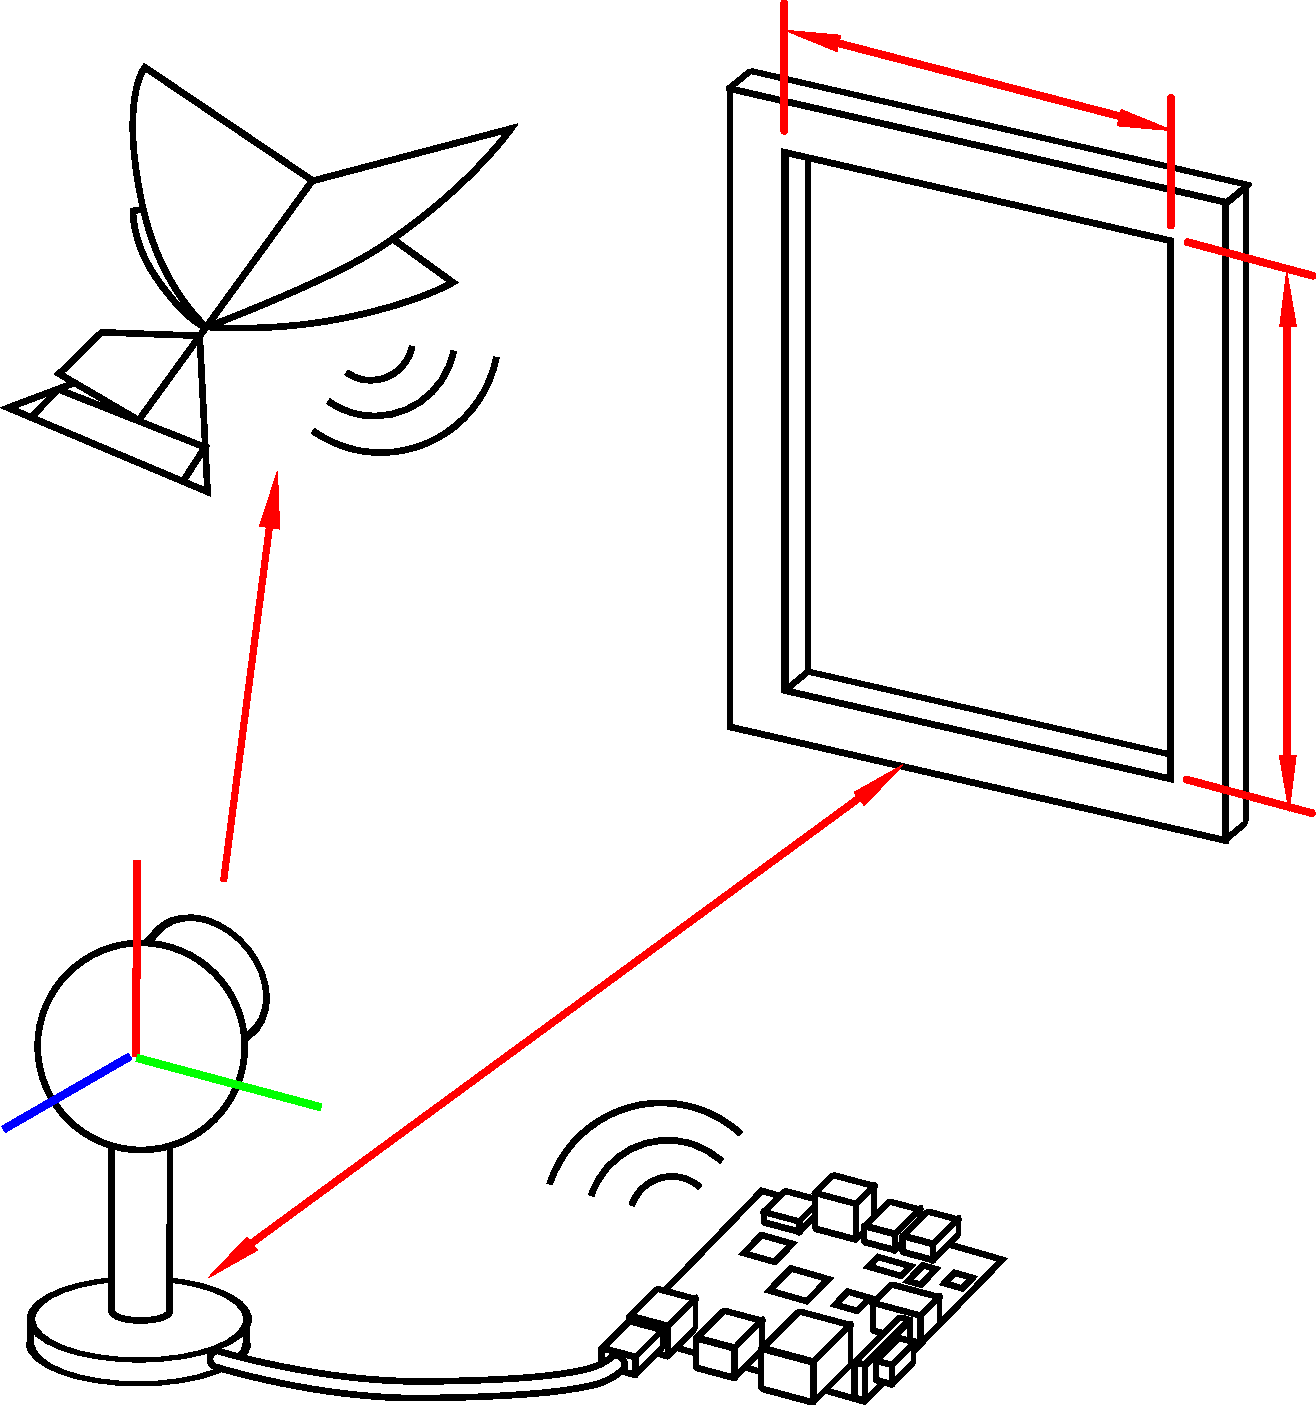
\includegraphics[width=\linewidth]{figures/experiment_cartoon.pdf}
\caption{Conceptual sketch of experimental environment.}
\label{fig:experiment_cartoon}
\end{figure}
%TODO label experiment cartoon

%%%%%%%%%%%%%%%%%%%%%%%%%%%%%%%%%%%%%%%%%%%%%%%%%%%%%%%%%%%%%%%%%%%%%%%%%%%%%%

%%%%%%%%%%%%%%%%%%%%%%%%%%%%%%%%%%%%%%%%%%%%%%%%%%%%%%%%%%%%%%%%%%%%%%%%%%%%%%
\section{Results and Performance}
\label{sec:performance}
%TODO cameron
To bound the performance of the cooperative control system, we determine 
the feasible set of initial conditions that result in successful narrow 
passage traversal using both analytical and empirical methods. We conducted 
experiments to validate this model.

The following sections detail how we calculated the feasible and infeasible
regions using system identification and present the results of our
experimental trials.

%----------------------------------------------------------------------------%
\subsection{System Identification}

%............................................................................%
\subsubsection{Ornithoper Attitude Control}
\label{sec:flight_control}
%TODO cameron
\begin{figure}[tb]
\centering
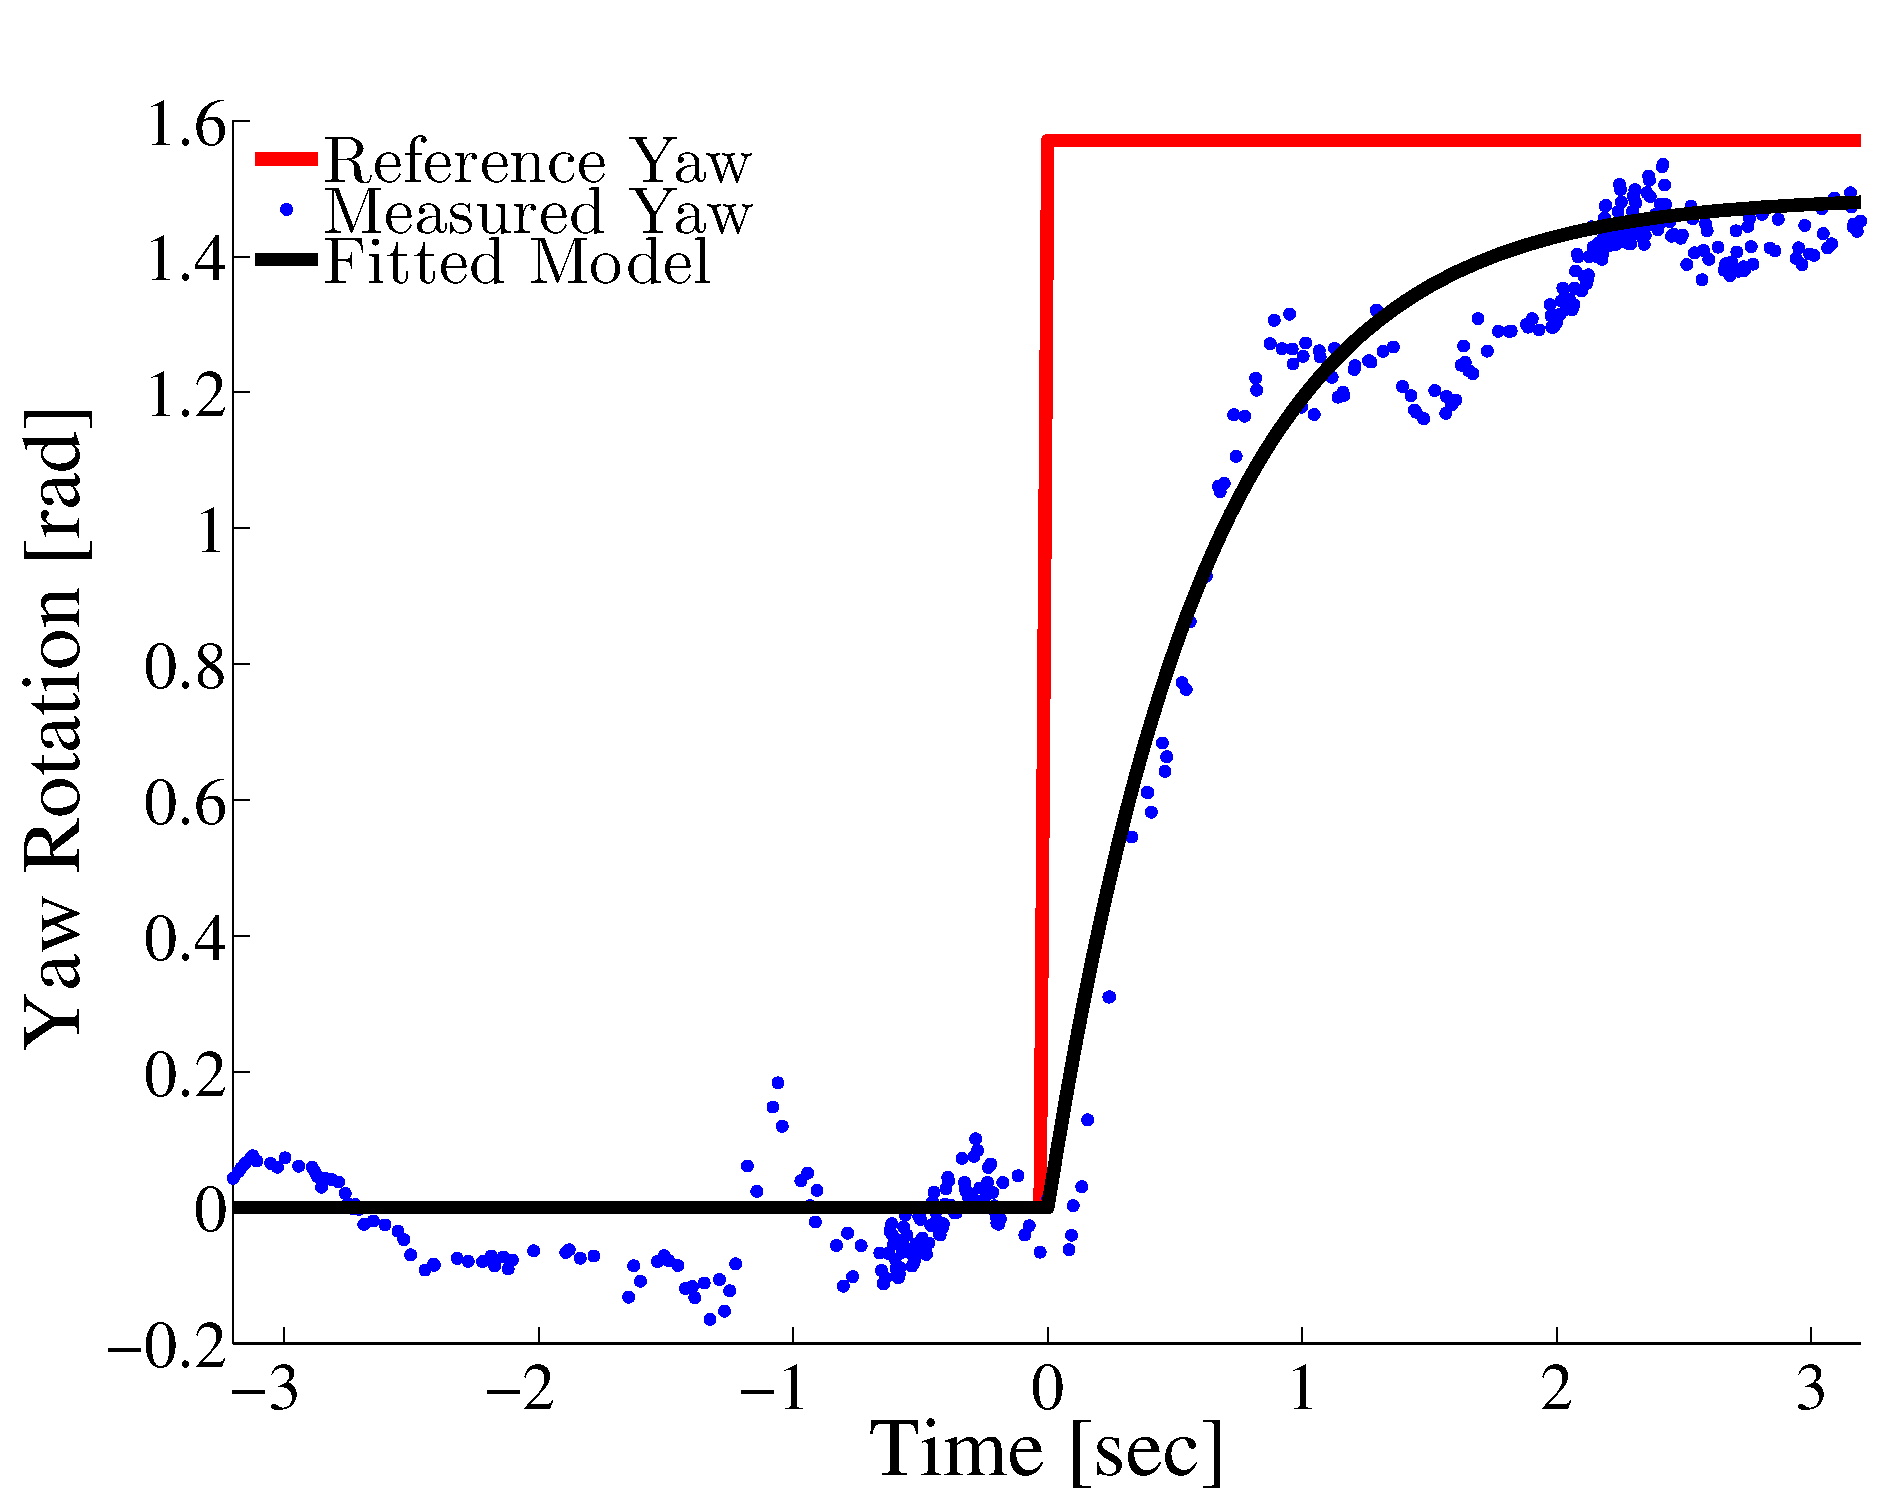
\includegraphics[width=\linewidth]{figures/step_response_total.pdf}
\caption{H$^2$Bird step response}
\label{fig:step_response}
\end{figure}
%TODO reduce number of sig figs

We depict the results of this experiment in
Figure~\ref{fig:step_response}. 

\begin{equation}
\label{eq:transfer_func}
H(s) = \frac{0.95}{1+0.62s}
\end{equation}
%TODO H(s) in a labeled equation
%TODO footnote for MATLAB

The step response rise time is approximately 1.4 seconds. The H$^2$Bird
flies at an average forward velocity of 1.2 m/s, so the estimated minimum
turning radius of the robot is 1.07 meters. In experiments, we choose a flight
speed lower than the maximum speed of the ornithopter, to facilitate more
robust tracking.


%TODO equation(s) for how you arrive at the minimum turning radius
%TODO footnote for MATLAB

%............................................................................%
\subsubsection{Ground Station Pose Estimation}

%............................................................................%
\subsubsection{Cooperative Visual Servoing}
\label{sec:visual_servoing}
%TODO cameron

%TODO make these span the page, with identical scales/style

\begin{figure*}[tb]
\begin{minipage}[b]{0.45\linewidth}
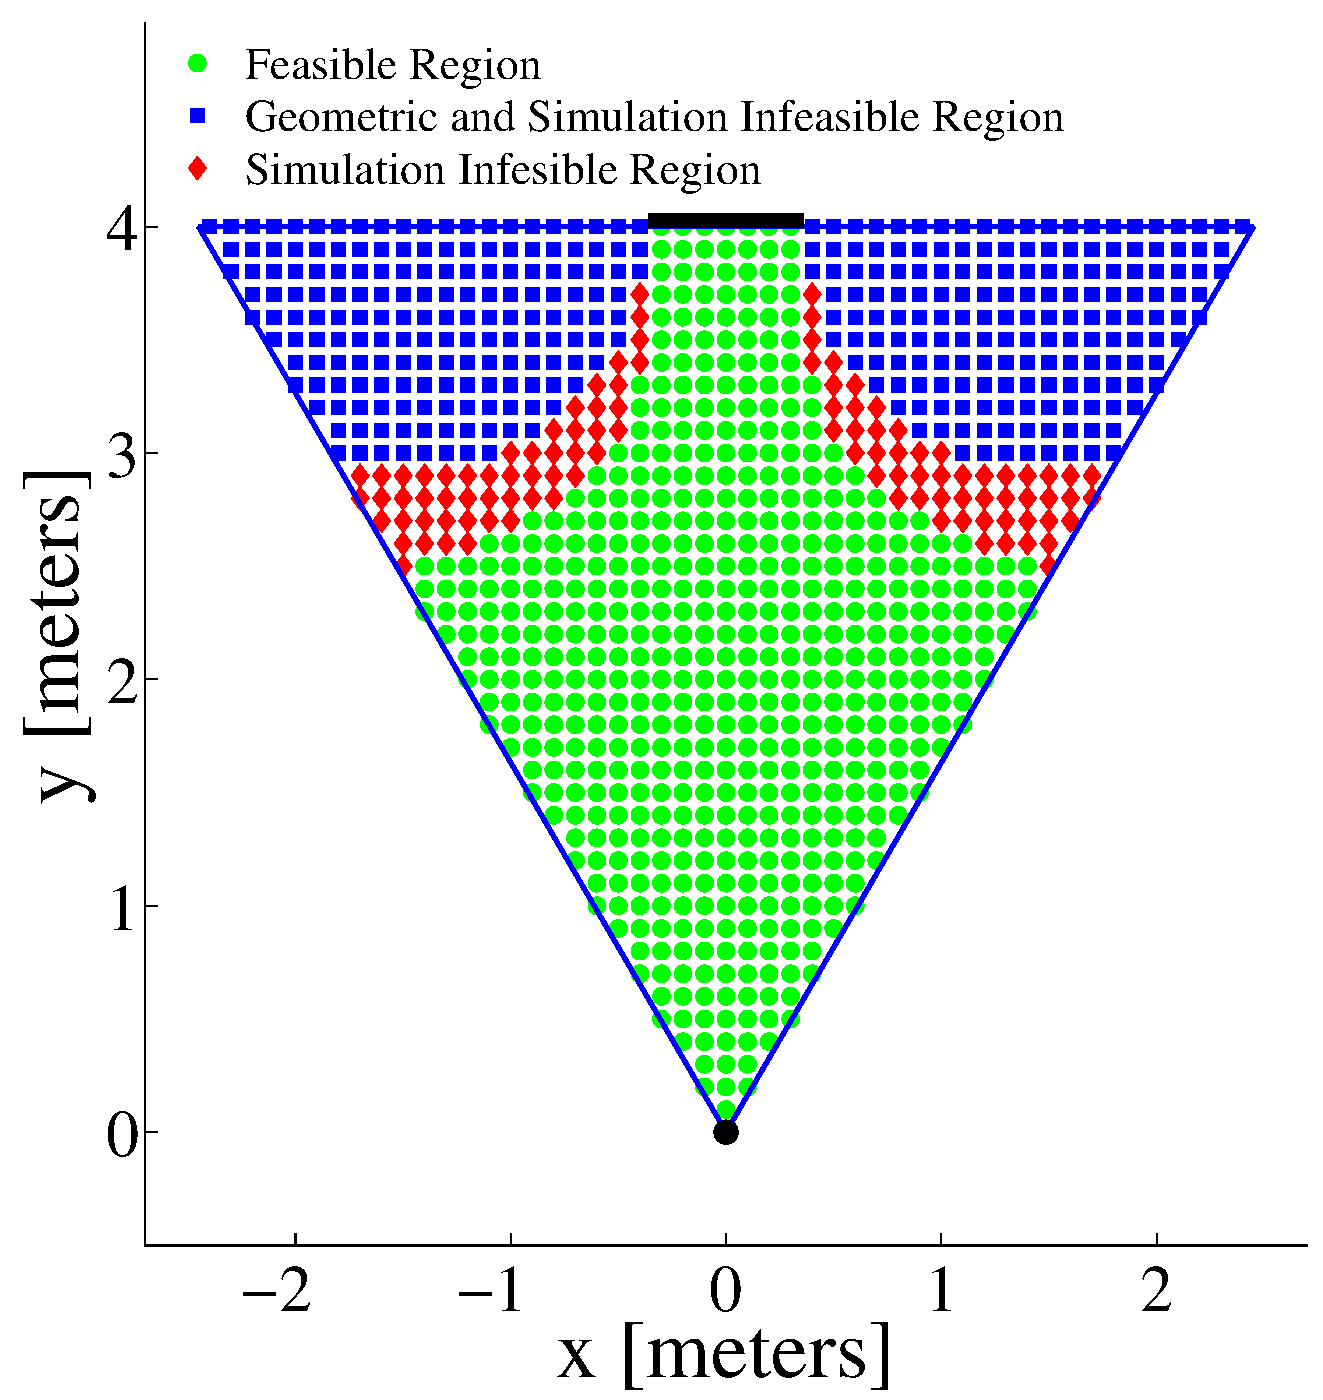
\includegraphics[width=\textwidth]{figures/feasible_set.pdf}
\caption{Plot of backwards reachable set for successful window traversal.}
\label{fig:feasible_set}
\end{minipage}
\hfill
\begin{minipage}[b]{0.45\linewidth}
\centering
\centering
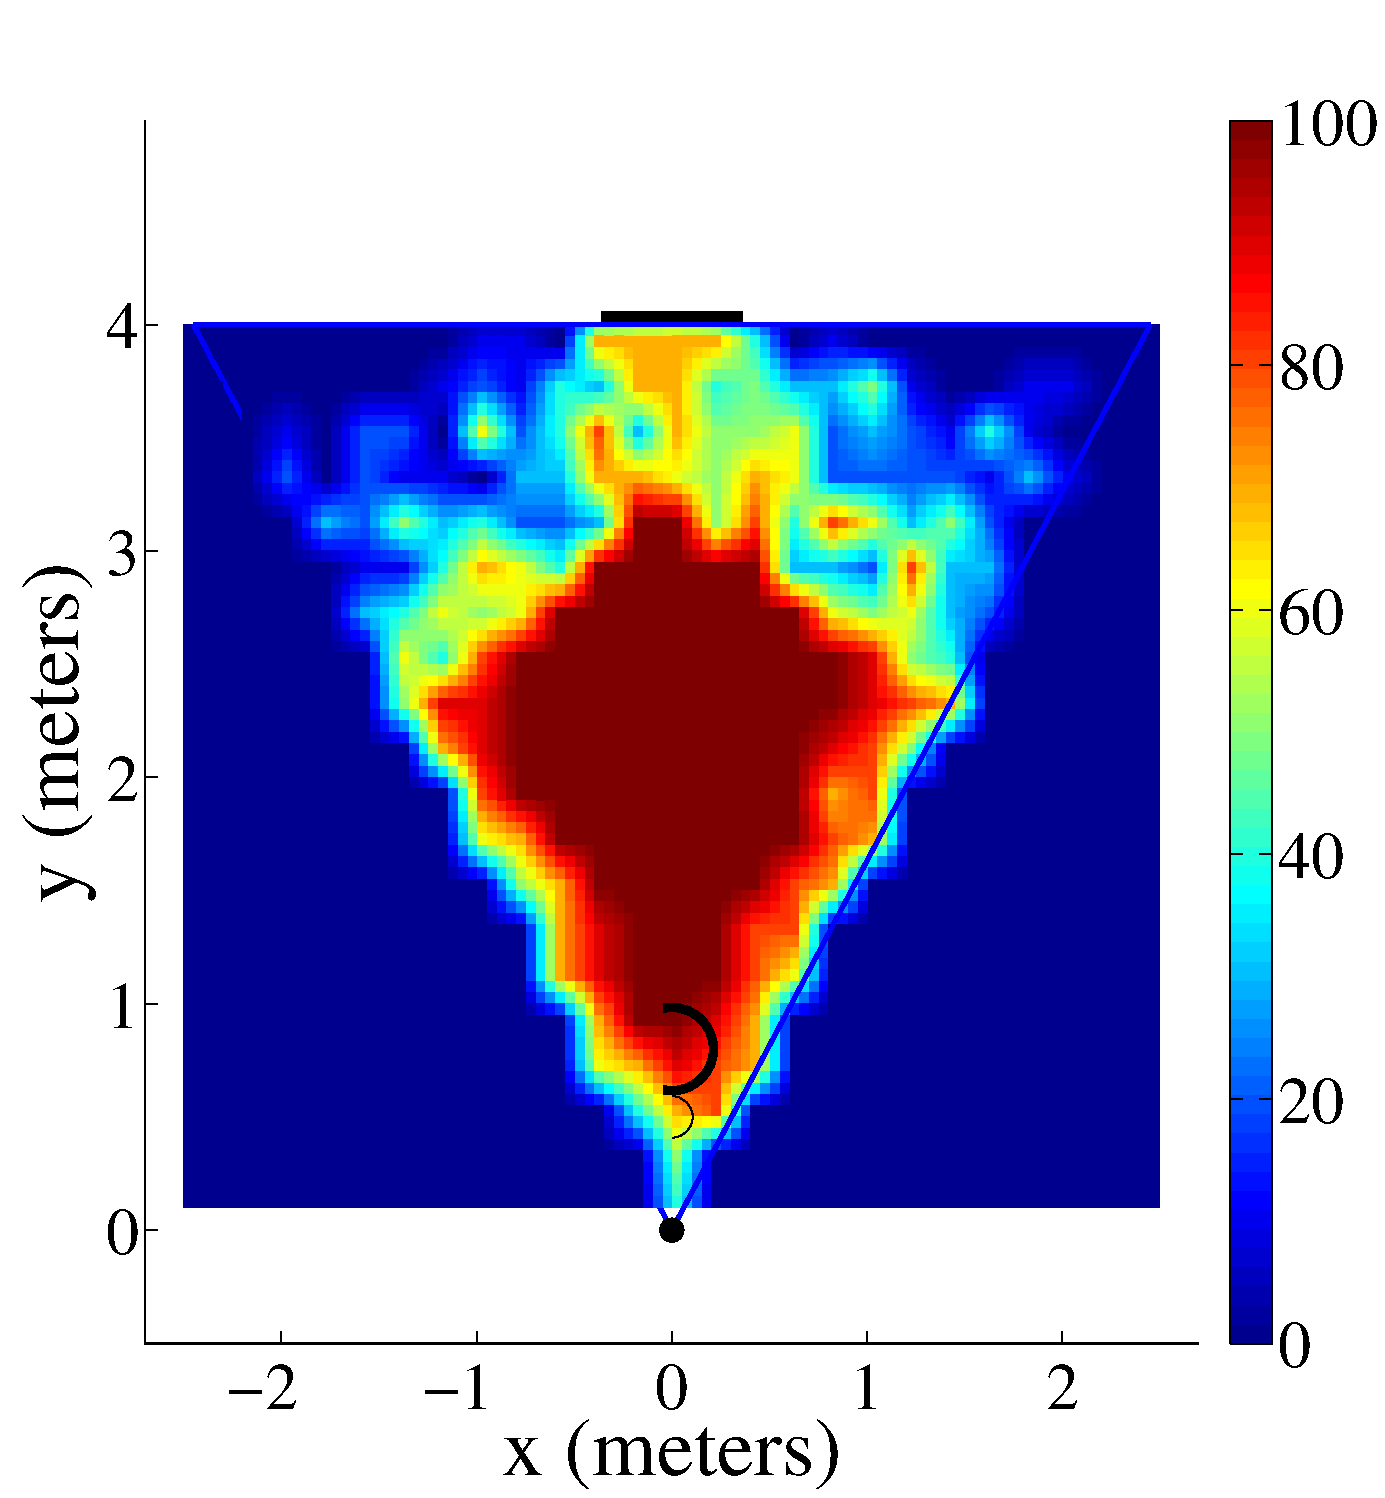
\includegraphics[width=\textwidth]{figures/heat_map.pdf}
\caption{Probability of success for all starting locations. This graphic is 
a result of a Monte Carlo simulation of the reachable set model, in which the 
initial heading of the H$^2$Bird is chosen uniformly at random from $(-90,90)$.}
\label{fig:heat_map}
\end{minipage}
\end{figure*}

\begin{figure*}[tb]
\begin{minipage}[b]{0.45\linewidth}
\centering
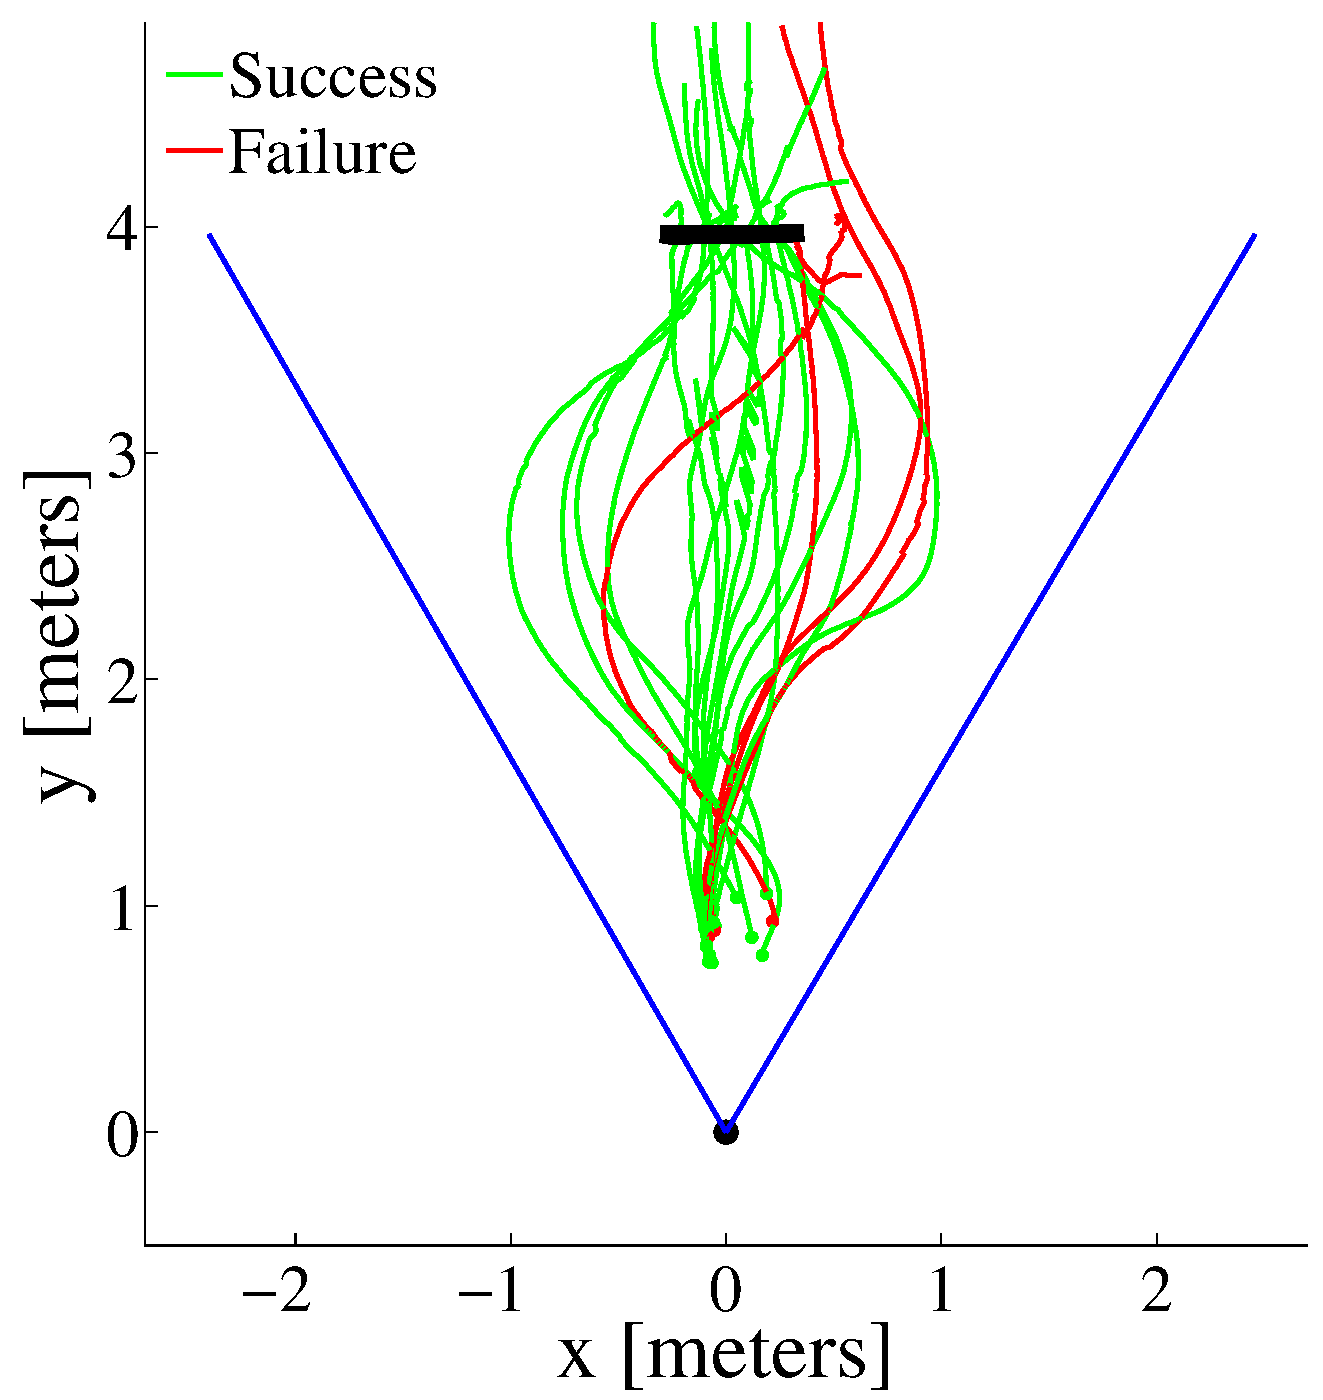
\includegraphics[width=\linewidth]{figures/flight_paths_feasible.pdf}
\caption{Plot of camera field of view and experimental trials within the feasible region.}
\label{fig:flight_paths_feasible}
\end{minipage}
\hfill
\begin{minipage}[b]{0.45\linewidth}
\centering
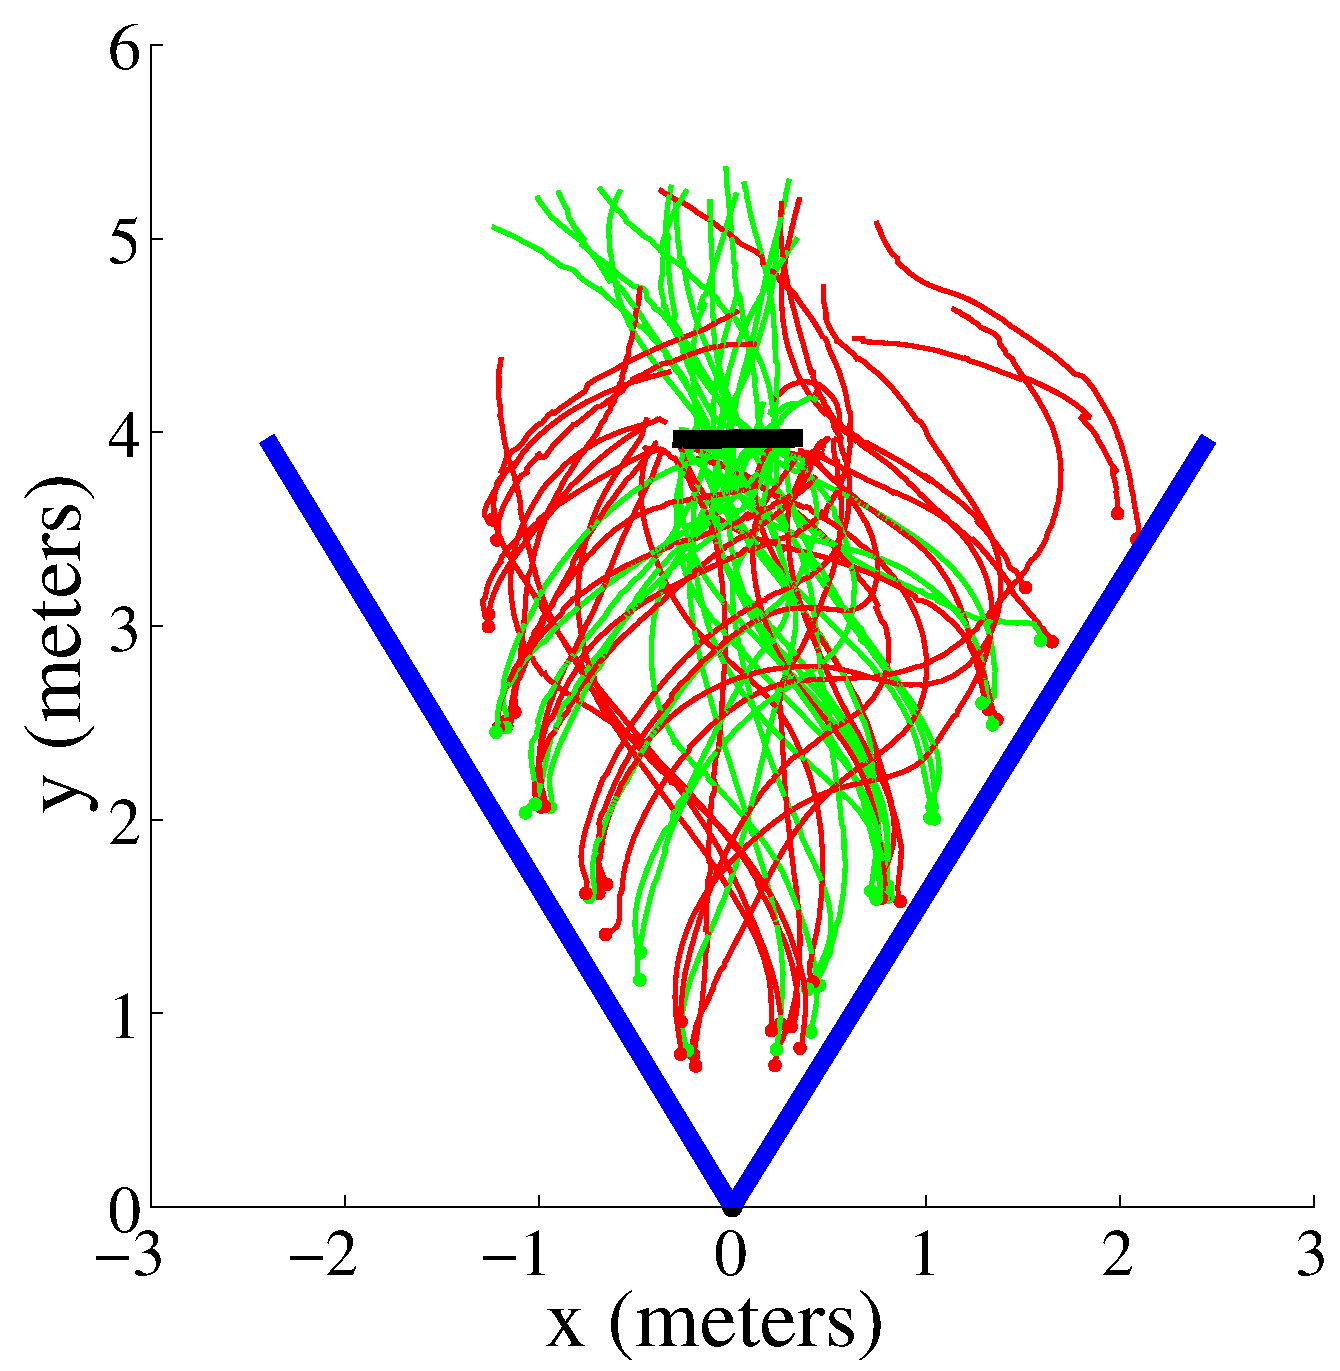
\includegraphics[width=\textwidth]{figures/flight_paths.pdf}
\caption{Plot of camera field-of-view and perimeter experimental trials overlayed.}
\label{fig:flight_paths}
\end{minipage}
\end{figure*}

The geometrically infeasible region is computed using the minimum
turning radius and the geometry of the camera's field-of-view. Both the 
regions in red and blue indicate the infeasible region determined in simulation. 
We ran a simulation on a motion model similar to Dubin's car in ~\cite{lavalle:planning}, with the
angular heading as the input rather than the angular velocity. We used the
turning model, described in Section~\ref{sec:flight_control}, as the input to
the motion model, with a PID controller steering the entire system to the
center of the passage as the input to the tuning model. 

We determine the backwards reachable set of initial states for successful
narrow passage traversal both geometrically and in simulation 
(Fig.~\ref{fig:feasible_set}). For the initial conditions, we use a uniform 
grid of 0.05 meter increments within the camera viewing region, and an 
initial angular position perpendicular to the narrow passage plane. 

The infeasible region
calculated in simulation is a superset of the geometrically infeasible region.
The simulation is more realistic as the rotational damping during the turn and
the on-board PID controller cause the real system to react to inputs at a
non-constant angular velocity.

The results of the experiments are shown in
Figures~\ref{fig:flight_paths} and~\ref{fig:flight_paths_feasible}.

%----------------------------------------------------------------------------%
\subsection{Model Verification}

For initial conditions in the middle of the feasible region and in front of
the camera, we achieved a success rate of 80\%. This case is depicted in
Figure~\ref{fig:flight_paths_feasible}. As we moved towards the edges of the
feasible region in Figure~\ref{fig:flight_paths}, the success rate diminishes
because of several factors. On the edges of the camera frame, the yaw control
inputs are large in magnitude, although this is not necessary in all cases.
Since the control algorithm we are using has no notion of depth, it applies
the same control input whether the ornithopter is close to the camera, where
small changes in heading are adequate, or far away from the camera, where
large changes in heading are necessary. Due to this phenomenon, the controller
often over- or under-compensates in certain regions, depending upon the PID
tuning and the distance from the camera. Tracking noise can also cause passage
negotiation to fail.

%%%%%%%%%%%%%%%%%%%%%%%%%%%%%%%%%%%%%%%%%%%%%%%%%%%%%%%%%%%%%%%%%%%%%%%%%%%%%%
\section{Conclusions and Future Work}
%TODO ryan
%%%%%%%%%%%%%%%%%%%%%%%%%%%%%%%%%%%%%%%%%%%%%%%%%%%%%%%%%%%%%%%%%%%%%%%%%%%%%%
\section{Acknowledgements}
The authors would like to thank Fernando Garcia Bermudez for his 
assistance with the Vicon motion capture system, Andrew Pullin for his 
help with robot photography, and the members of the Biomimetic 
Millisystems Laboratory and the EECS community at the University of 
California, Berkeley for their advice and support.

%%%%%%%%%%%%%%%%%%%%%%%%%%%%%%%%%%%%%%%%%%%%%%%%%%%%%%%%%%%%%%%%%%%%%%%%%%%%%%%

%%%%%%%%%%%%%%%%%%%%%%%%%%%%%%%%%%%%%%%%%%%%%%%%%%%%%%%%%%%%%%%%%%%%%%%%%%%%%%%
% BIBLIOGRAPHY

% The following two commands are all you need in the
% initial runs of your .tex file to
% produce the bibliography for the citations in your paper.
\bibliographystyle{abbrv}
\bibliography{manuscript}

% ACM needs 'a single self-contained file'!
%\subsection{References}
% Generated by bibtex from your ~.bib file.  Run latex,
% then bibtex, then latex twice (to resolve references)
% to create the ~.bbl file.  Insert that ~.bbl file into
% the .tex source file and comment out
% the command \texttt{{\char'134}thebibliography}.
\end{document}
